\documentclass{egpubl}
\usepackage{eurovis2023}
\EuroVisShort  % for EuroVis additional material
\usepackage[T1]{fontenc}
\usepackage{dfadobe}  
\usepackage{cite}  % comment out for biblatex with backend=biber
\BibtexOrBiblatex
\electronicVersion
\PrintedOrElectronic
\ifpdf \usepackage[pdftex]{graphicx} \pdfcompresslevel=9
\else \usepackage[dvips]{graphicx} \fi
\usepackage{egweblnk}
\usepackage{todonotes}  % Custom package for add notes
\usepackage{subcaption}


\title[]%
      {Analyzing Travel Distance and Environmental Impact in the Formula 1 World Championship Calendar}

\author[Luca Anzaldi, Massimo Giaccone, Martin Heywang \& Himanshu Sharma]
{\parbox{\textwidth}{\centering L. Anzaldi$^{1}$, M. Giaccone$^{1}$, M. Heywang$^{1}$ and H. Sharma $^{1}$
        }
        \\
{\parbox{\textwidth}{\centering $^1$University of Southern Denmark, Odense, Denmark}
}
}


%-------------------------------------------------------------------------
\begin{document}

% uncomment for using teaser
% \teaser{
%  \includegraphics[width=\linewidth]{eg_new}
%  \centering
%   \caption{New EG Logo}
% \label{fig:teaser}
%}

\maketitle
%-------------------------------------------------------------------------
\begin{abstract}

Formula 1 championships involve one of the most complex logistical operations in modern sport, requiring the transportation of cars, equipment, and personnel across multiple continents within a single season. While the environmental impact of Formula 1 has received increasing attention in recent years, the inefficiencies generated by the ordering of races in the official calendar are often discussed only qualitatively. This project investigates unnecessary travel produced by the current Formula 1 race calendar by visualizing the geographic distribution of circuits and quantifying distances between consecutive events. Using historical circuit data and geographic coordinates, we compute travel distances across full championship seasons and estimate environmental impact by combining distance metrics with publicly available freight emission factors.

We implement an optimization pipeline that reorders races to minimize total travel distance and compare the optimized route to the official calendar. To support transparency, the system exposes emission coefficients (truck and air) and explicitly separates truck and flight distances when calculating totals. Interactive visualizations include a world map with route overlays, comparative summaries, and a carbon dashboard that distinguishes per-season views from multi-year trends. Additional views quantify intercontinental jumps per season and the split between truck and flight emissions. The findings highlight persistent back-and-forth movements that increase travel distance and estimated emissions. By making these inefficiencies visible and comparable, this work demonstrates how visualization and optimization can support informed discussion about sustainability in global sports logistics and the consequences of calendar design.

\end{abstract}  
%-------------------------------------------------------------------------
\section{Introduction}

Formula 1 is one of the most globally distributed sporting events in the world, with a championship calendar spanning multiple continents over the course of a single season. Each year, teams, equipment and personnel are transported across thousands of kilometers to reach more than twenty race locations worldwide. While the sport is often associated with technological innovation and high performance, its global logistics operation represents a significant and often overlooked source of environmental impact.

In recent seasons, the Formula 1 calendar has raised concerns due to apparent inefficiencies in race scheduling. Events are sometimes organized in a sequence that requires teams to travel back and forth between distant regions, such as moving from the Middle East to North America and then back to Europe within a short time span. These scheduling choices increase total travel distance, logistics complexity, and associated carbon emissions, even when alternative race orders could reduce unnecessary movement.

Logistics in Formula~1 are extremely demanding and represent one of the most complex operational systems in global sport. Each season involves transporting cars, garage equipment, spare parts, and personnel across five continents using a combination of air freight, sea freight, and road transport. According to official sustainability reports, Formula~1 logistics rely heavily on air cargo, with hundreds of tons of equipment moved between events using large cargo aircraft operated by logistics partners such as DHL~\cite{F1Sustainability2025}.

Publicly available logistics analyses indicate that a single race event may require up to six or seven Boeing~747 cargo aircraft, while over a season teams collectively ship approximately 660 tons of air freight and 500 tons of sea freight~\cite{F1LogisticsDHL}. In addition, hundreds of trucks are used to transport equipment between geographically closer races, forming convoys several kilometers long. While recent sustainability initiatives aim to reduce emissions, the global scale of the championship makes travel-related environmental impact a persistent challenge.

Previous discussions around Formula 1 sustainability have largely focused on power unit efficiency, fuel innovation, and on-track emissions. Comparatively less attention has been paid to the structure of the race calendar itself and the cumulative impact of long distance travel between events. Understanding how calendar design influences total travel distance is therefore essential for evaluating potential improvements in the sport’s environmental footprint.

The goal of this project is to use data visualization to explore and quantify travel inefficiencies in Formula 1 championship calendars. By mapping circuit locations and analyzing distances between consecutive races, we aim to provide an intuitive and data-driven representation of global movement throughout a season. Additionally, we estimate the environmental impact of this travel by combining distance measures with logistics and emissions data reported in sustainability studies.

Beyond analyzing the current calendar, this work also explores hypothetical optimized race sequences designed to minimize total travel distance. By comparing the actual and optimized calendars, the project highlights the potential reduction in travel and environmental impact achievable through alternative scheduling strategies. Interactive visualizations are used to support exploration, comparison, and user-driven analysis, making complex logistical patterns more accessible and interpretable.

Historical information about circuits, race calendars, and locations is obtained from a publicly available dataset covering Formula~1 seasons from 1950 to 2025~\cite{f1dataset}.

%-------------------------------------------------------------------------
\section{Related Work}

Research on sports logistics and sustainability has investigated the environmental costs of global event schedules, often focusing on transport emissions and calendar efficiency. Prior work in logistics optimization typically frames scheduling as a routing or traveling-salesperson problem with additional constraints, while visualization research emphasizes the value of geographic overviews and comparative path representations for communicating complex movement patterns. In the Formula~1 context, public sustainability reports and analyses provide estimates of freight emissions and qualitative discussion of travel inefficiencies~\cite{F1Sustainability2025,F1LogisticsDHL}, but they rarely connect route order to explicit, visually comparable travel paths.

Our work contributes a focused visualization system that combines geographic route comparison with interactive optimization and emissions estimation. Unlike static analyses, the system enables users to explore specific seasons, adjust emission parameters, and compare optimized versus official calendars. The result is an application that supports exploratory reasoning about schedule design choices and their environmental implications rather than a single, fixed optimization outcome.


%-------------------------------------------------------------------------
\section{Design}
\label{sec:design}

The design of our system is guided by the objective of supporting exploratory visual analysis of Formula~1 race calendars, using historical circuit and race data collected from publicly available sources~\cite{f1dataset}.
The interface is conceived as a flexible analytical environment in which users can freely navigate across views and progressively refine their understanding. In the following, we describe the design choices of the system by structuring the discussion around the \emph{What}, \emph{Why}, and \emph{How} of the interface.

\subsection{What: System Functionality}

The system is an interactive visual analytics application that enables users to explore Formula~1 circuits and race calendars at a global scale. Its main functionalities include:
\begin{itemize}
    \item a world map providing an overview of all Formula~1 circuits;
    \item visualization of race sequences as geographic paths connecting circuits in calendar order;
    \item comparison between the original race calendar and an optimized alternative path aimed at reducing travel distance and associated CO$_2$ emissions;
    \item access to detailed circuit information, including geographic context and historical statistics;
    \item user-controlled parameters for estimating environmental impact, such as emission coefficients for different transportation modes;
    \item a carbon dashboard that separates per-season analysis from multi-year trends and includes derived metrics such as intercontinental jumps and truck-vs-flight emission splits.
\end{itemize}

Together, these features allow users to analyze both the spatial distribution of Formula~1 races and the implications of calendar ordering on travel efficiency and sustainability.

\subsection{Why: Design Rationale}

\subsubsection{Exploratory Analysis and User Goals.}
The primary goal of the system is to support exploratory analysis rather than task-oriented interaction. Users are not expected to follow a predefined workflow, but instead to investigate the data from multiple perspectives, compare alternatives, and develop insights through interaction. For this reason, the interface does not impose a strict navigation flow; instead, it allows users to switch freely between views such as circuits, races, and optimized paths according to their analytical needs.

\subsubsection{Overview and Progressive Disclosure.}
The design is inspired by the Information Seeking Mantra~\cite{InformationSeeking}: \emph{overview first, zoom and filter, then details on demand}. The world map provides an immediate overview of all circuits, while zooming and filtering operations allow users to focus on specific seasons or subsets of races. Detailed information about circuits and race sequences is revealed only when needed, reducing initial visual complexity and cognitive load.

\subsection{How: Interface Implementation}

The core of the interface is an interactive world map that serves as the primary entry point for exploration. Circuits are represented as map markers, while race sequences are visualized as curved paths to preserve geographic continuity and improve readability at different zoom levels. Optimized paths are displayed using distinct visual encodings to facilitate comparison with the original calendar. The map view allows users to select subsets of races and immediately see how the route and computed totals change.
The system is also designed to be modular and extensible, enabling future refinements and additional analytical features without requiring fundamental changes to the interaction paradigm.

\subsubsection{Color and Visual Encoding}
A coherent and limited color palette inspired by Formula~1 visual identity is adopted across the interface to ensure consistency and recognizability. Neutral tones are used for geographic context, while more saturated colors highlight analytical elements such as race paths and optimized routes. Different hues are employed to distinguish original and optimized calendars, enabling direct visual comparison. Although multiple colors appear across maps and charts, this redundancy is intentional and serves to reinforce semantic distinctions across different views.  

\subsubsection{Redundancy and Information Reinforcement}
The system intentionally introduces a degree of information redundancy, for example by presenting circuit information both in dedicated circuit views and within race-related contexts. This choice is motivated by established principles in information visualization, where redundancy can improve usability by reducing the need for users to mentally integrate information across distant views. By reinforcing key concepts in multiple locations, the interface supports faster comprehension and lowers the risk of misinterpretation.

\subsubsection{Interaction Design Choices}
Interaction is based on direct manipulation techniques such as hovering, clicking, and selection to support incremental and transparent exploration. Hovering reveals labels and contextual information only when needed, reducing visual clutter in dense geographic regions, while selection enables users to progressively construct subsets of races for optimization. User-defined parameters, including emission coefficients, support what-if analyses by directly influencing optimization outcomes. Environmental impact estimates combine inter-circuit travel distances with air and truck emission factors, following internationally recognized aviation emission methodologies from the International Civil Aviation Organization (ICAO)~\cite{ICAOCalculatorAirFreight,ICAOCalculatorMethodology}, ensuring consistency and methodological transparency across comparisons.

\subsubsection{Distance estimation}
Distance estimation is designed to be interpretable and consistent across views. We compute leg distances from geographic coordinates and separate truck versus flight contributions for local versus intercontinental moves. This enables direct visual comparison between calendar ordering, travel distance, and emissions impact without introducing opaque transformations. The resulting distances are stored in a yearly data table that the application loads on demand.

\subsubsection{Optimization algorithm}
The optimization algorithm (\autoref{fig:pseudocode-graph-opt}) combines a nearest-neighbor heuristic with a 2-opt improvement step. This approach produces a coherent route while keeping computation fast enough for interactive use. 


\begin{figure}
    \centering
    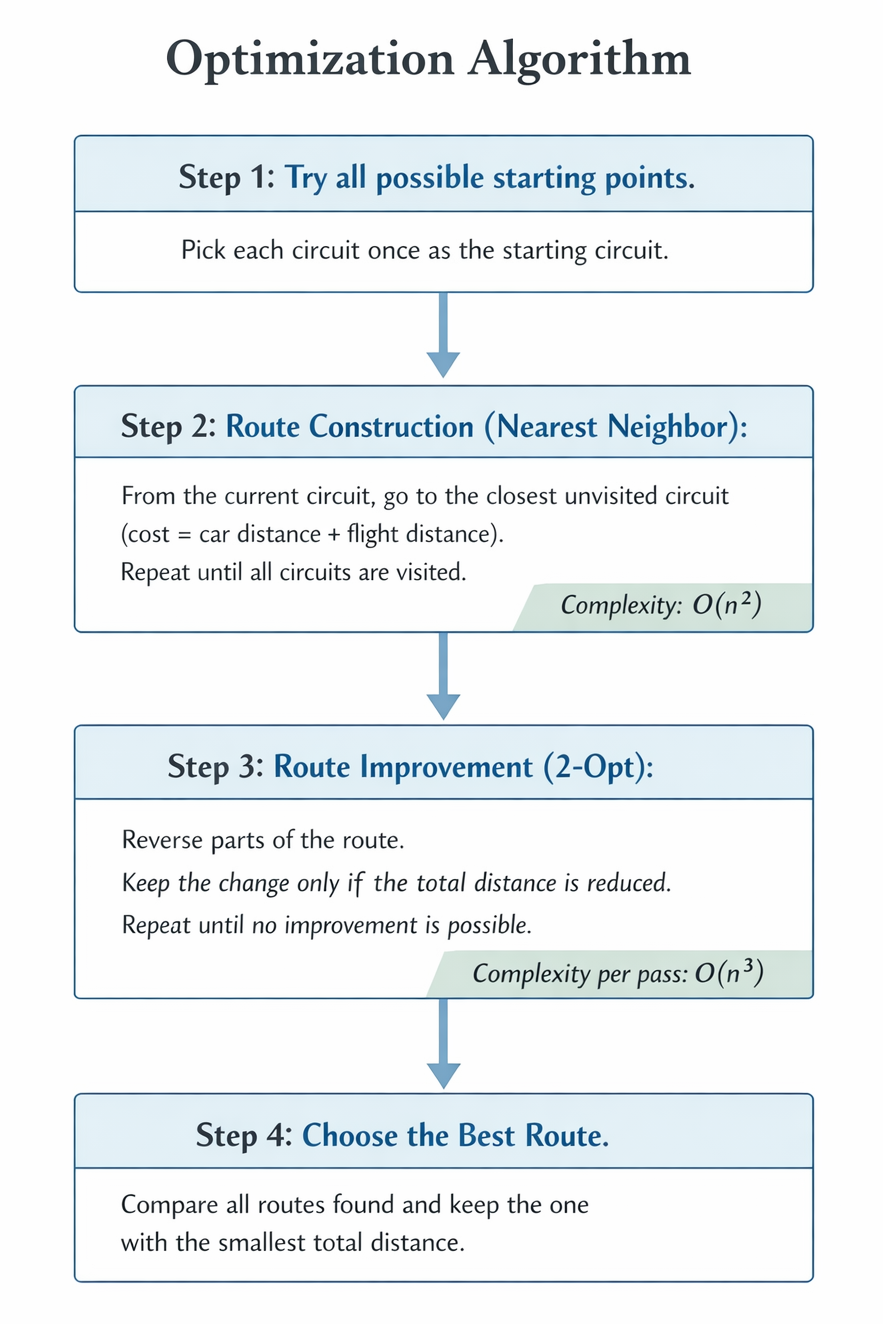
\includegraphics[width=\linewidth]{images/Opt_algorithm.png}
    \caption{Pseudocode: optimization algorithm}
    \label{fig:pseudocode-graph-opt}
\end{figure}





%-------------------------------------------------------------------------
\section{Results}
\label{sec:results}

The results of our project are primarily qualitative and exploratory, supported by quantitative estimations of travel distance and environmental impact. The system enables users to visually and interactively compare the official Formula~1 race calendar with an optimized alternative, highlighting inefficiencies in the original scheduling.

\subsection{Geographic Patterns in the Official Calendar.}
Figure~\ref{fig:calendar_comparison}(a) shows the original race calendar for a selected season, visualized as a sequence of geographic paths connecting consecutive circuits. The visualization reveals a recurrent pattern of long intercontinental jumps, often followed by returns to previously visited regions. In several seasons, races alternate between distant continents such as Europe, the Middle East, and North America, producing extensive back-and-forth travel. While such patterns may be driven by commercial or organizational constraints, their spatial implications become immediately apparent through the map-based representation.

\subsection{Optimized Calendar and Reduced Travel}
Figure~\ref{fig:calendar_comparison}(b) presents the optimized race calendar generated by reordering events to minimize total travel distance. Compared to the original schedule, the optimized path exhibits a more geographically coherent structure, grouping races by region and reducing the number of long-distance transitions. The visual difference between the two paths clearly illustrates how alternative scheduling strategies could significantly reduce unnecessary travel.

\subsection{Environmental Impact Estimation}
By combining geographic distance with user-defined emission coefficients, the system provides an estimate of the environmental impact associated with each calendar configuration. Although these estimates rely on simplified assumptions and do not aim to be exact measurements, they follow internationally recognized emission calculation practices~\cite{FuelBurnCommercialJets,ICAOCalculatorAirFreight}. This makes them suitable for comparative analysis between alternative calendar configurations.


\subsection{Exploratory Interaction and Insight Generation}
An important outcome of the project is the ability for users to actively explore different scenarios. By selecting subsets of races or adjusting emission parameters, users can observe how small changes influence the overall travel pattern and environmental impact. This interactive process supports hypothesis generation rather than definitive conclusions, encouraging users to reflect on the trade-offs involved in global sporting event logistics.

\subsection{Summary of Findings}
Overall, the results indicate that the current Formula~1 calendar contains structural inefficiencies from a geographic and environmental perspective. Through visual comparison and interactive optimization, our system demonstrates that alternative race orderings could substantially reduce travel distances and associated emissions, without altering the set of host circuits.

\begin{figure}[tbp]
  \centering

  \begin{subfigure}{\linewidth}
    \centering
    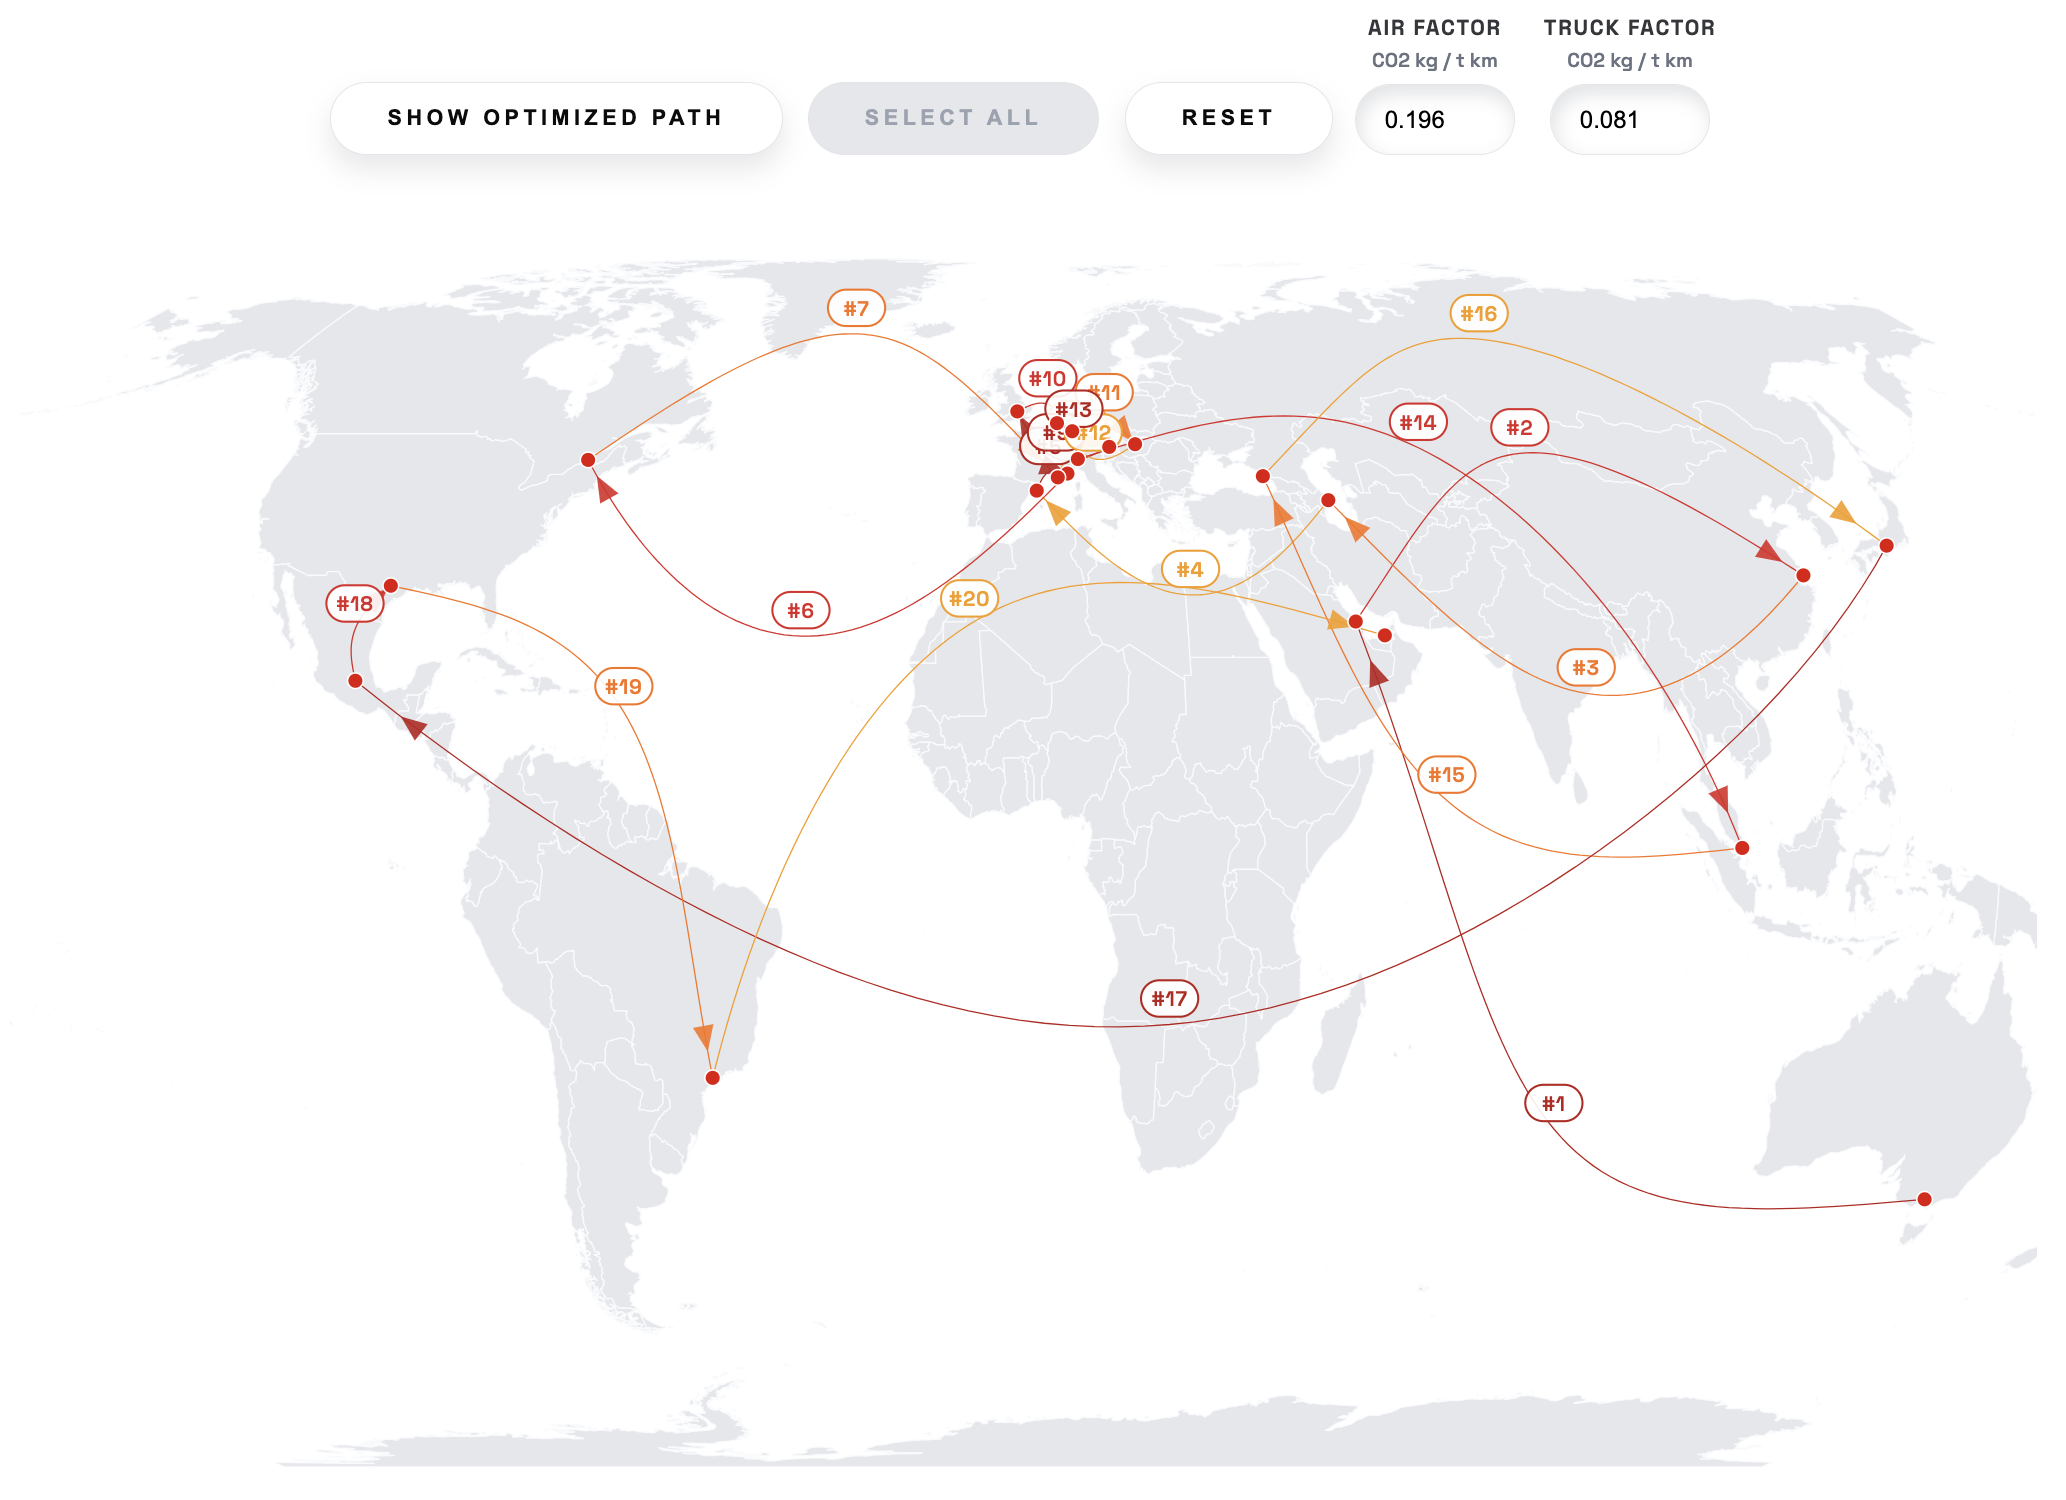
\includegraphics[width=\linewidth]{images/fig1.png}
    \caption{Original Formula~1 race calendar}
    \label{fig:calendar_original}
  \end{subfigure}

  \vspace{0.5cm}

  \begin{subfigure}{\linewidth}
    \centering
    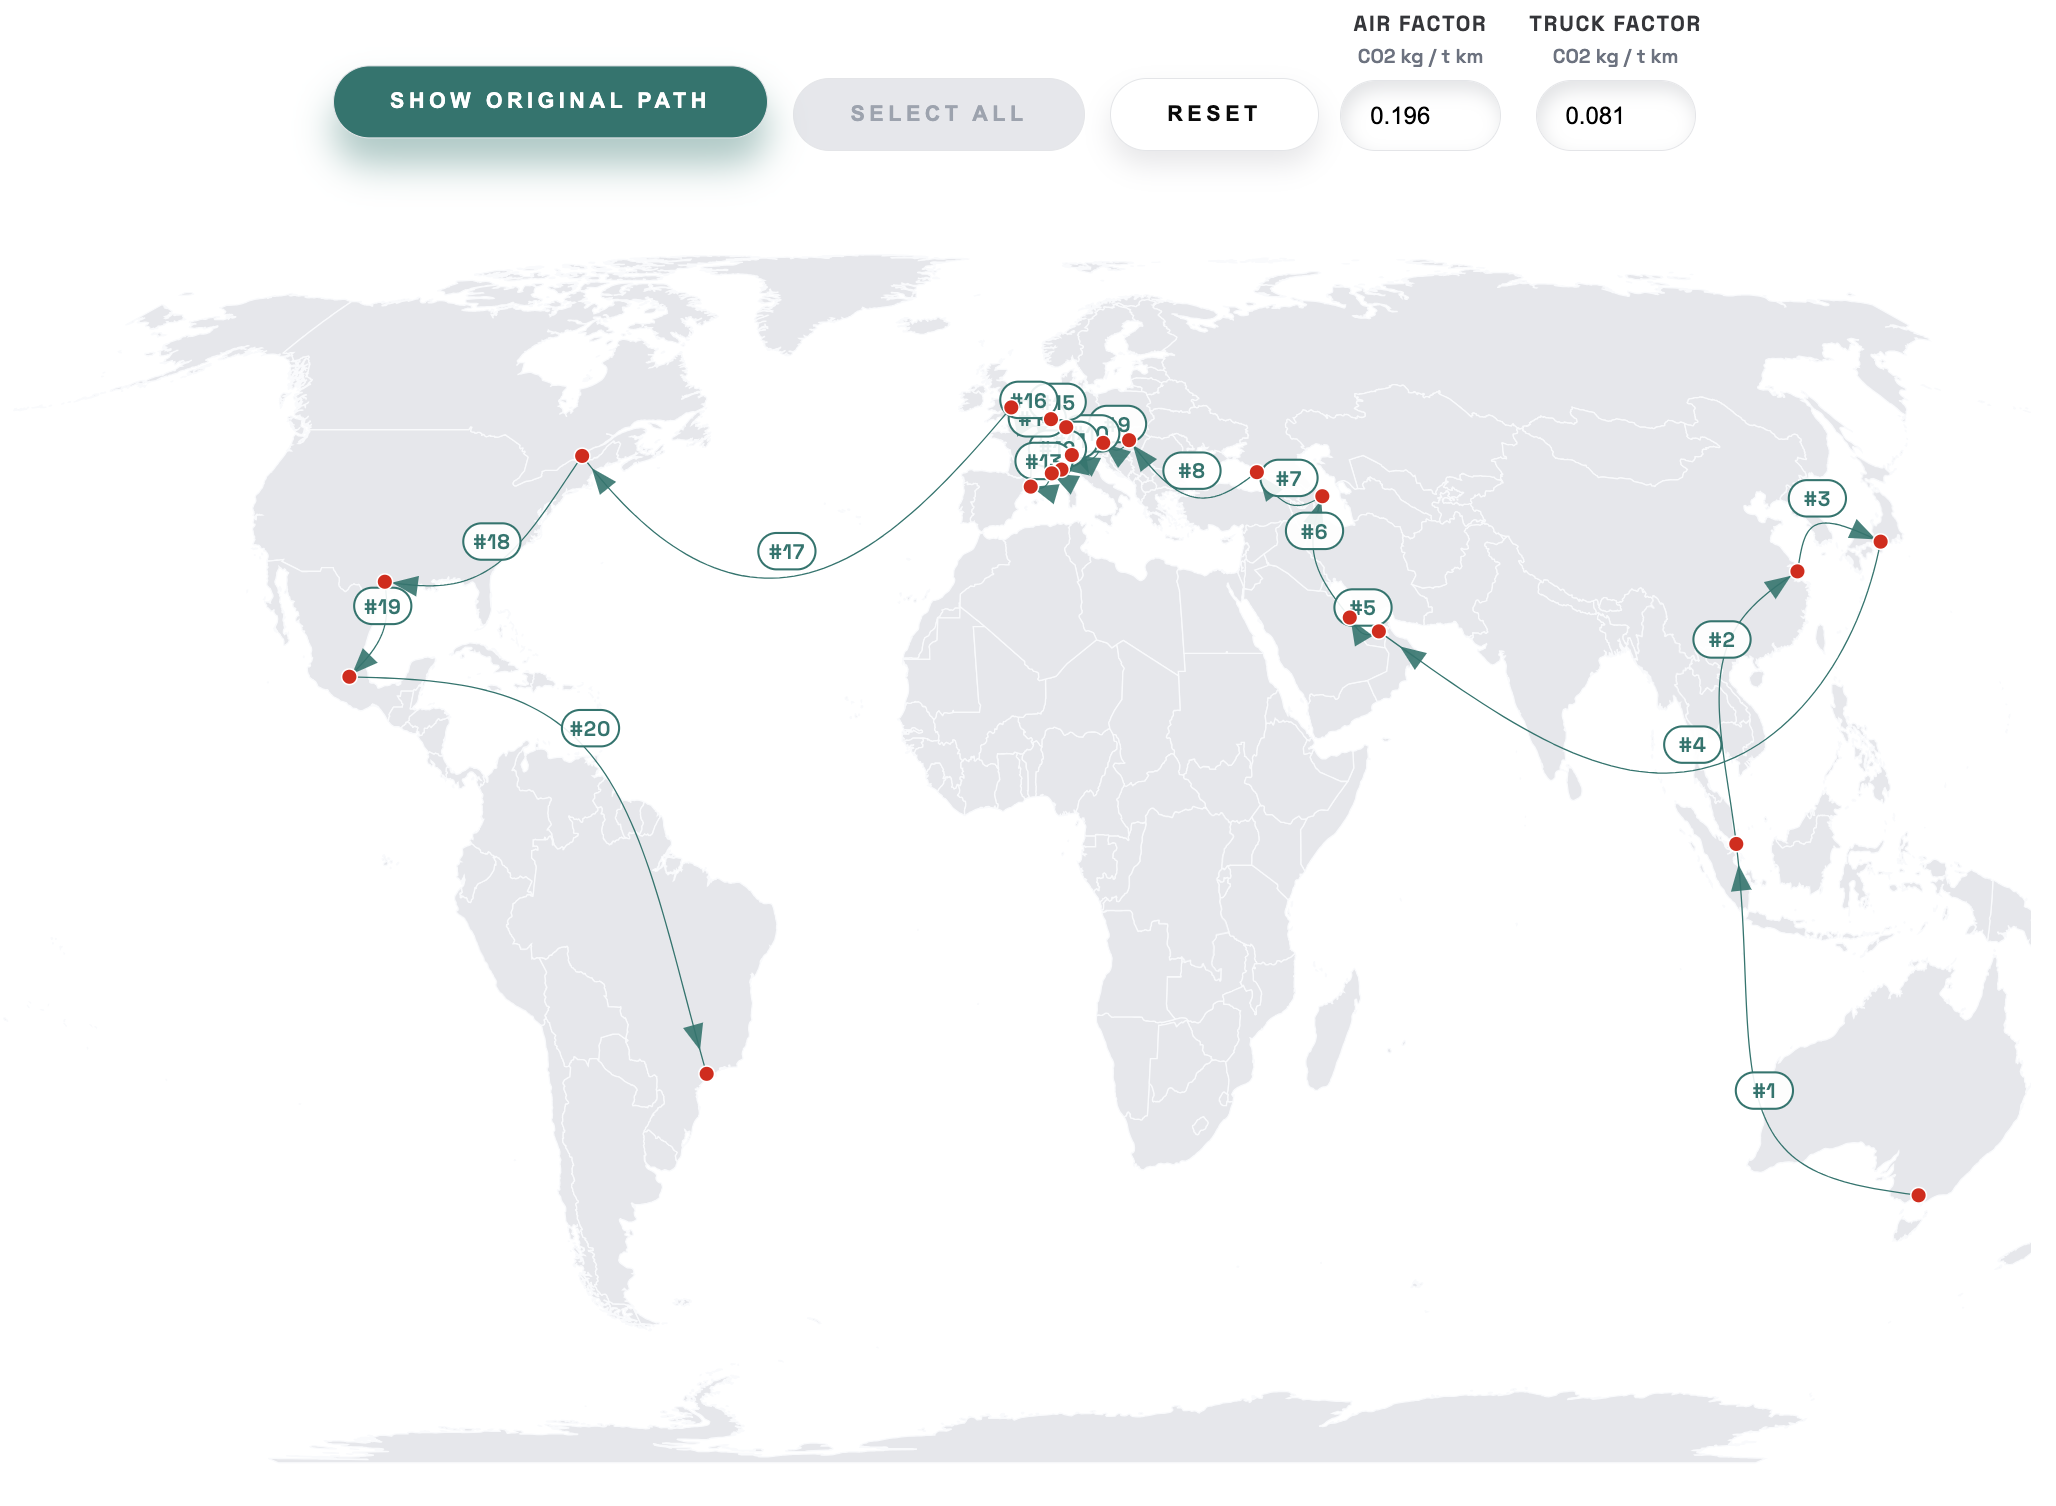
\includegraphics[width=\linewidth]{images/fig2.png}
    \caption{Optimized Formula~1 race calendar}
    \label{fig:calendar_optimized}
  \end{subfigure}

  \caption{Comparison between the original Formula~1 race calendar (a) and the optimized calendar (b) for a selected season. The optimized path reduces long intercontinental transitions and results in a more geographically coherent sequence of races.}
  \label{fig:calendar_comparison}
\end{figure}




%-------------------------------------------------------------------------
\section{Conclusion}
\label{sec:conclusion}

In this project, we explored the geographic and environmental implications of the Formula~1 race calendar through an interactive visual analytics system. By combining map-based visualizations with distance estimation and simple environmental impact models, we provided users with tools to analyze and compare the official championship schedule against alternative, optimized race orderings.

Our results highlight that the current Formula~1 calendar often involves \textit{significant unnecessary travel}, characterized by frequent intercontinental back-and-forth movements. Through visual comparison and optimization, we demonstrated that reordering races while preserving the same set of host circuits can substantially reduce total travel distance and estimated CO$_2$ emissions. These findings suggest that calendar structure plays a crucial role in the sustainability of global sporting events.

Beyond the specific Formula~1 use case, this work emphasizes the value of interactive geospatial visualization for understanding complex logistical systems. The system is designed to support exploratory analysis rather than to produce definitive numerical predictions, encouraging users to reflect on trade-offs between organizational constraints, geographic efficiency, and environmental impact.

While the current implementation relies on simplified assumptions and does not account for all real-world constraints of race organization, it provides a solid foundation for further investigation. Future extensions could incorporate more detailed logistics data (e.g., actual freight routing and sea freight schedules), stronger environmental models, and tighter integration between race scheduling and operational constraints.

Although the proposed model relies on simplified assumptions, it follows internationally recognized methodologies for aviation emission estimation~\cite{ICAOCalculatorMethodology}. This allows the system to effectively communicate relative differences in travel-related environmental impact, supporting informed discussion rather than precise prediction.

Overall, the project demonstrates how visual analytics can make abstract sustainability issues tangible and accessible, fostering awareness and informed discussion about the environmental costs of large-scale international events.

%-------------------------------------------------------------------------
% References
\bibliographystyle{eg-alpha-doi}
\bibliography{references}

\end{document}
